Der nun behandelte temporale Algorithmus von \cite{hal02158423} beruht 
im Gegensatz zu \cite{georgiev2016blue} auf \textit{nachträglichen} 
Annahmen. Welches zur Folge hat, dass die Dimension unseres Path Tracers
\nameref{ch:Content1:sec:Path Tracer}, sowie die Stichprobenanzahl einhergehen 
mit der Verteilung der Integrationsfehler als blue noise im Bildraum.
Die zu Grunde liegenden Annahmen sollen nun im Folgenden untersucht werden.

\subsection{Theoretische Grundlage}

Im Kapitel \nameref{ch:Content1:sec:Path Tracer} haben wir gesehen, dass 
wir den Wert eines Pixels (i,j) klassischerweise mit einem zufälligen
Startwert durch eine Monte-Carlo Integration erhalten. Wir betrachten im
Folgenden eine (theoretische) Menge von allen möglichen Werten eines 
Pixels, welche durch alle möglichen Startwerte generiert wurde.
In \nameref{eq:Pixel Schätzung Wahrscheinlichkeitsdichtefunktion} ist die Wahrscheinlichkeitsdichtefunktion
$h_{ij}$ aufgetragen, als eine Funktion über alle möglichen Werte 
$I_{ij}$ eines Pixels (i,j).

\begin{equation}\label{eq:Pixel Schätzung Wahrscheinlichkeitsdichtefunktion}
    H_{ij}([I_{Anfang},I_{Ende}]) = \int_{I_{Anfang}}^{I_{Ende}} h_{ij} dI
\end{equation}

Verfolgt man beispielhaft die Werte eines Pixels über 9 frames bei unseren Path Tracer 
basierend auf \cite{Benty18}, so ergibt es sich zur Anschauung wie folgt:

\begin{figure}[H]

    \begin{subfigure}{\textwidth}
        \centering 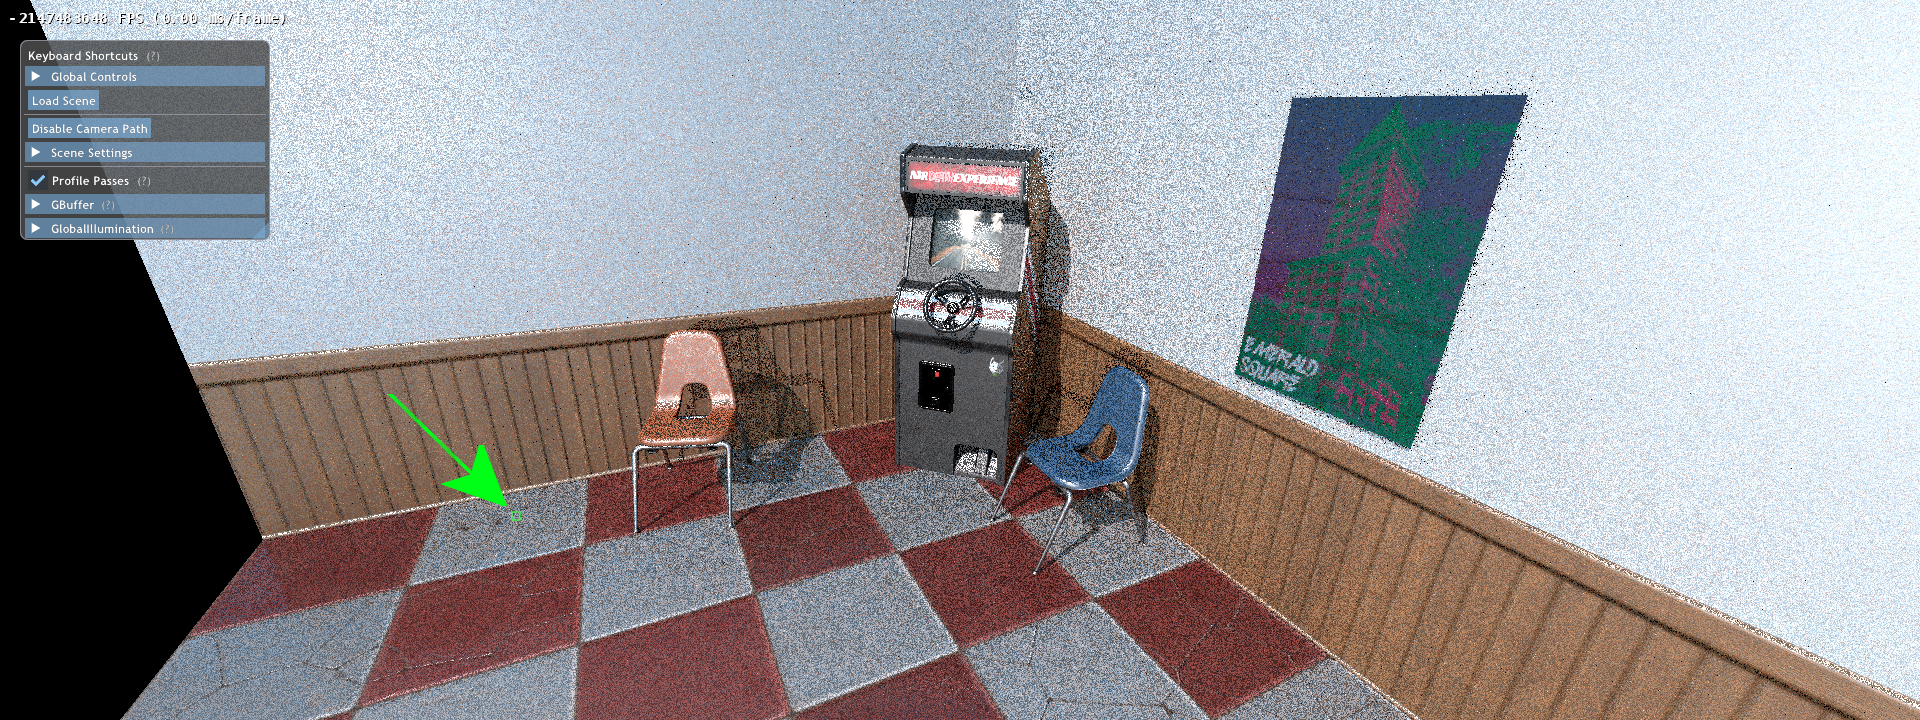
\includegraphics[width=0.6\linewidth]{content/TemporalerAlg/Bilder/APosteriori/frame_t_whitenosie2.0.png} 
        \caption{Szenenausschnitt}
        \label{fig:szene_pixel_position_512x512}
    \end{subfigure}

    \begin{subfigure}{0.5\textwidth}
        \centering 
\includegraphics[width=0.6\linewidth]{content/TemporalerAlg/Bilder/APosteriori/pixel_512x512_strip.png} 
        \caption{Werte des Pixels an Position 512x512 im zeitlichen Verlauf (Rote Markierung)}
        \label{fig:ausschnitt_pixelstrip}
    \end{subfigure}
    \begin{subfigure}{0.5\textwidth}
            \centering
            \def\svgwidth{\columnwidth}
            \import{content/TemporalerAlg/Bilder/APosteriori/}{histogram_of_estimates.pdf_tex}
            \label{histogramOfEstimates}
            \caption{Histogram der Pixelschätzungen}
    \end{subfigure}
        \caption{Pixelwerte an Position 512x512(grüne Markierung) in aufeinanderfolgenden Zeitschritten}
        \label{fig:Pixelwerte}

\end{figure}

Allerding betrachten wir die theoretische Menge aller Werte. Demnach können wir das Rendern 
eines jeden konkreten Pixels als die Wahl eines Wertes anhand der Wahrscheinlichkeitsdichtefunktion
sehen.

Daraus lässt sich die Gleichbedeutung zweier Aussagen begründen:
Das Rendern des Pixels (i,j) und das Wählen eines Pixelswertes $I_{ij}$
von unser zuvor formulierten Wahrscheinlichkeitsdichtefunktion $h_{ij}$.

\begin{equation}\label{eq:inverse Funktion}
    I_{ij} = H_{ij}^{-1}(x), x \in [0,1]
\end{equation}

Nun betrachte man die Werte für x in \nameref{eq:inverse Funktion} als im Bildraum
blue noise verteilte Zahlen. Daraus folgt, dass die resultierenden
Integrationsfehler auch als blue noise im Bildraum verteilt sind.


\subsection{Praktische Durchführung}
Die Berechnung des vollständigen Histogramms ist für eine Echtzeitanwendung
zu kostenintensiv. Stattdessen könnte man auch die dadurch beanspruchte 
Rechenleistung auf z.B mehrere Samples pro Pixel verteilen.
Stattdessen werden wir in dem temporalen Algorithmus von \cite{hal02158423}
das Histogramm mit dem vorherigen Frame approximieren. 
Bereits vorherige Arbeiten \cite{Schied:2018:GER:3273023.3233301} haben die 
Wirksamkeit eines solchen temporalen Ansatzes(Zugriff auf das vorherige Frame)
gezeigt. Die Approximation des Histogramms erfolgt dadurch mit dem $Frame_{t}$ 
für $Frame_{t+1}$,indem umliegende Pixel in das Histogramm aufgenommen werden.
Offensichtliche Konsequenzen dieser blockweisen Verarbeitung sind schlechte blue noise 
Fehlerverteilungen im Bildraum bei sich stark ändernden Bildausschnitten
(so z.B. bei Objektkanten), da dort die Annahme, dass eine ähnliche Oberfläche
zur Farbgebung beiträgt verletzt wird.


\begin{algorithm}[H]
    \caption{Benutzung unser zwei vorberechneten Texturen: Blue Noise und Retarget}
    \begin{algorithmic}[1]
        \State $bluenoise_{t}$(i,j) = $bluenoise_{0}$(i + $\alpha$t, j + $\beta$t); 
        \State $retarget_{t}$(i,j) = $retarget_{0}$(i + $\alpha$t, j + $\beta$t) + ($\alpha$t, $\beta$t)
    \end{algorithmic}
    \label{alg:Benutzung vorberechneter Texturen}
\end{algorithm}

\begin{figure}[H]
    \centering
    \begin{subfigure}[b]{0.4\textwidth}
        \centering 
\includegraphics[interpolate=false, width=\linewidth]{content/TemporalerAlg/Bilder/APosteriori/homogener_ausschnitt_blocksize.png}
        \label{fig:homogener Pixelblock}
        \caption{homogener Pixelblock}
    \end{subfigure}
    ~ %add desired spacing between images, e. g. ~, \quad, \qquad, \hfill etc. 
      %(or a blank line to force the subfigure onto a new line)
    \begin{subfigure}[b]{0.4\textwidth}
        \centering 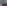
\includegraphics[interpolate=false,width=\linewidth]{content/TemporalerAlg/Bilder/APosteriori/inhomogener_ausschnitt_blocksize.png}
        \label{fig:Inhomogener Pixelblock}
        \caption{inhomogener Pixelblock}
    \end{subfigure}

    \caption{Pixelblöcke bei (in-)homogenen Flächen}\label{fig:Pixelblöcke}
\end{figure}